\documentclass[12pt]{scrartcl} %Dokumentklasse, bestimmt Teile des Layouts
\usepackage{Pre} % importiert das .syt-File


\begin{document}

%----------------------------------------------------------------------------

\begin{titlepage}
\begin{center}
\vspace*{2cm}
\begin{LARGE}
\vspace*{1cm}
\textbf{\textsf{Versuch 7: Redoxreaktionen\\}}
\end{LARGE}
\vspace*{1cm}
\textbf{\textsf{Integriertes Praktikum ROR}}\\
\vspace*{1.5cm}


\begin{table}[H]
\sffamily

\hspace*{3cm}\begin{tabular}{>{\bfseries}l>{\bfseries}l}
Verfasser 1: & Victor Schneider\\
Matrikelnummer 1: & 3715169\\
E-Mail-Adresse 1: & st188901@stud.uni-stuttgart.de\\
Verfasser 2: & Vincent Peters\\
Matrikelnummer 2: & 3841428\\
E-Mail-Adresse 2: & st200821@stud.uni-stuttgart.de\\
\end{tabular}
\vspace{1cm}

\hspace*{3cm}\begin{tabular}{>{\bfseries}l>{\bfseries}l}
    Gruppe: & 2a \\
    Assistent: & Frank Zimmer
\end{tabular}
\vspace{1cm}

\hspace*{3cm}\begin{tabular}{>{\bfseries}l>{\bfseries}l}
   Versuchsdatum: & 04.05.2026 \\
   Abgabedatum 1: & 08.05.2026 \\ 
\end{tabular}
\end{table}
\end{center}

\end{titlepage}


\renewcommand{\thepage}{\Roman{page}}\setcounter{page}{1}
\tableofcontents %Generiert ein Inhaltsverzeichnis, optional
\newpage
\renewcommand{\thepage}{\arabic{page}}\setcounter{page}{1}

%____________________________________________________________________________

\section{Theorie}
\subsection{Redoxreaktion}
Eine Redoxreaktion ist eine Elektronenübertragungsreaktion. Dabei wird ein Stoff oxidiert, das heißt er gibt Elektronen ab und ein Stoff wird reduziert, er nimmt Elektronen auf. Dabei ändern sich die Oxidationszahlen. 
Der Stoff der als Oxidationsmittel reagiert, oxidiert den anderen und wird dabei selbst reduziert, er nimmt also Elektronen auf. Im Gegensatz dazu wird der Stoff, der als Reduktionsmittel reagiert selbst oxidiert und gibt somit Elektronen ab. Es kann nie eine Reduktion ohne Oxidation oder eine Oxidation ohne Reduktion stattfinden \cite{skript}.

\subsection{Elektrochemische Spannungsreihe}
Jeder Stoff hat ein unterschiedlich hohes Bestreben Elektronen aufzunehmen oder abzugeben. Dieses Bestreben ist das Redoxpotential. Da dieses Potential nicht direkt gemessen werden kann, muss es gegen eine Referenz, die Standard-Wasserstoffelektrode (SHE) gemessen werden. Definiert ist hier das Gleichgewicht zwischen Wasserstoff und Oxonium-Ionen $\ce{H2 <=> 2 H+}$. Stoffe mit positivem Redoxpotential reagieren im Bezug auf dieses Redoxpaar als Oxidationsmittel, Stoffe mit negativen Redoxpotential als Reduktionsmittel. Die Redoxpotentiale von Stoffen bei Standartbedingungen (1013 mbar, 298,15 K und 1 $\frac{\text{mol}}{\text{L}})$ sind in der elektrochemischen Spannungsreihe geordnet. Die Potentiale einzelner Redoxpaare können bei nicht-Standartbedingungen über die Nernstsche Gleichung berechnet werden: \cite{skript}
\begin{equation}
    E = E^0 + \frac{\text{R} \cdot T}{z \cdot \text{F}} \cdot \ln{\frac{c_{ox}}{c_{red}}}
\end{equation}

Dafür werden die ideale Gaskonstante $\text{R} = 8,314 \,\text{J} \cdot \text{mol}^{-1} \cdot \text{K}^{-1}$, die Temperatur $T$, die Ladungszahl $z$, die Faraday-Konstante $\text{F} = 96485\,\text{C} \cdot \text{mol}^{-1}$ sowie die Konzentrationen $c_{ox}$ und $c_{red}$ benötigt.


\newpage


\subsection{Komproportionierung und Disproportionierung}
Reagiert das gleiche Element aus verschiedenen Verbindungen in der gleichen Oxidationsstufe miteinander, besteht die Möglichkeit, das Element in Verbindung 1 zu oxidieren und in Verbindung 2 zu reduzieren. Diese Art der Reaktion heißt Disproportionierung. Dabei teilt sich die Oxidationsstufe von einer mittleren zu einer höheren und einer niedrigeren.\\
Als Komproportionierung versteht man die Reaktion eines Elements, das in verschiedenen miteinander reagierenden Verbindungen in unterschiedlicher Oxidationsstufe vorliegt, zu einer Verbindung in der dieses Element in der gleichen Oxidationsstufe vorliegt.
\cite{skript}


% nicht cite vergessen :)
\section{Versuch 1: Elektrochemische Spannungsreihe}
\subsection{Aufgabenstellung}
Redoxpaare sollten untersucht und in die elektrochemische Spannungsreihe eingeordnet werden.




\subsection{Versuchsdurchführung}
Der Versuch bestand aus zwei Teilversuchen.\\
Im ersten Versuchsteil wurde verdünnte Salzsäure hergestellt und vier Reagenzgläser wurden damit befüllt. In die Reagenzgläser wurden jeweils etwas Magnesium, Nickel, Zink und Kupfer gegeben.\\[2mm]
Im zweiten Versuchsteil wurde zuerst verdünnte Salpetersäure hergestellt. Dann wurde etwas Zink in 3 Reagenzgläser gegeben. Die Reagenzgläser wurden jeweils mit etwas konzentrierter Salzsäure, verdünnter und konzentrierter Salpetersäure befüllt. Der Versuch wurde mit Kupfer statt Zink wiederholt.

\subsection{Beobachtungen}
Im ersten Versuchsteil konnte Gasbildung am Magnesium, Nickel und Zink beobachtet werden, wobei das Magnesium am kürzesten reagierte und das Nickel am längsten. Am Kupfer konnte keine Reaktion festgestellt werden.\newpage
Im zweiten Versuchsteil wurde bei der Reaktion des Zinks mit der konzentrierten Salzsäure ein weißes Gas gebildet, bei der Reaktion mit verdünnter Salzsäure ein hellbraunes Gas und bei der Reaktion mit konzentrierter Salzsäure ein braunes Gas. Das Kupfer reagierte nicht mit der konzentrierten Salzsäure. Bei der Reaktion mit verdünnter Salpetersäure bildetet sich ein hellbraunes Gas und die Lösung färbte sich türkis und bei der Reaktion mit konzentrierter Salpetersäure entstand ein braunes Gas und die Lösung färbte sich dunkeltürkis. Zudem liefen beide Reaktionen mit der verdünnten Salpetersäure langsamer ab als die Reaktionen mit der konzentrierten Salpetersäure.



\subsection{Auswertung}
Die Reaktionen der Metalle aus dem ersten Versuchsteil und des Zinks aus dem zweiten Versuchsteil mit Salzsäure laufen folgendermaßen ab: 
\begin{align}\notag
    &\text{Oxidation:} ~~ \ch{"\ox{0,Me}" _{(s)} -> "\ox{+2,Me}" _{(aq)}} \ce{ + 2e^-}\\\notag
    &\text{Reduktion:} ~~ \ch{2 "\ox{+1,H}" _{(aq)} +}\ce{2e^-} \ch{-> "\ox{0,H_2}" _{(g)} ^}\\\notag
    &\text{Gesamtreaktion:} ~~ \ch{"\ox{0,Me}" _{(s)}} + \ch{2 "\ox{+1,H}" _{(aq)} -> "\ox{+2,Me}" _{(aq)}} + \ch{"\ox{0,H_2}" _{(g)} ^}\\
\end{align}
Bei dem Gas, dass sich bei den Reaktionen bildete, handelte es sich also um Wasserstoff.\\

Die Reaktionen des Zinks und Kupfers mit der verdünnten Salpetersäure liefen folgendermaßen ab: 
\begin{align}\notag
    &\text{Oxidation:} ~~ \ch{"\ox{0,Me}" _{(s)} -> "\ox{+2,Me}" _{(aq)}} \ce{ + 2e^-}\\\notag
    &\text{Reduktion:} ~~ \ch{"\ox{5,N}" {}O3^{-}_{(aq)} + 4 H^+_{(aq)} + 3 e^{-} -> "\ox{2,N}" O{}_{(g)} ^ + 2 H2O_{(l)}}\\ \notag
    &\text{Gesamtreaktion:} ~~ \ch{3 "\ox{0,Me}" _{(s)} + 2 "\ox{5,N}" {}O3^{-}_{(aq)} + 8 H^+_{(aq)} -> 3 "\ox{+2,Me}" _{(aq)} + 2 "\ox{2,N}" O{}_{(g)} ^ + 4 H2O_{(l)}}\\
\end{align}


\newpage


Da bei den Reaktionen mit der verdünnten Salpetersäure ein braunes Gas beobachtet wurde kann es sich dabei nicht um Stickstoffmonoxid handeln, da dieses farblos ist. Das Stickstoffmonoxid muss also beim Austritt aus der Lösung mit dem Wasser zu Stickstoffdioxid reagiert sein. 
\begin{align}\notag
     &\text{Oxidation:} ~~ \ch{"\ox{+2,N}" O _{(g)} + H_2O _{(l)} -> "\ox{+4,N}" O_2 _{(g)} + 2 {H+} _{(aq)} + 2 {e^-}}\\\notag
    &\text{Reduktion:} ~~ \ch{"\ox{0,O_2}" _{(g)} + 4 {H^+} _{(aq)} + 4 {e^-} -> 2 H_2 "\ox{-2,O}" _{(l)}}\\\notag
    &\text{Gesamtreaktion:} ~~ \ch{2 "\ox{+2,N}" O _{(g)} + "\ox{0,O_2}" _{(g)} -> 2 "\ox{+4,N}" "\ox{-2,O_2}" _{(g)}}\\
\end{align}

Die Reaktionen des Zinks und Kupfers mit der konzentrierten Salpetersäure laufen folgendermaßen ab: 
\begin{align}\notag
    &\text{Oxidation:} ~~ \ch{"\ox{0,Me}" _{(s)} -> "\ox{+2,Me}" _{(s)}} \ce{ + 2e^-}\\ \notag
    &\text{Reduktion:} ~~ \ch{"\ox{5,N}" {}O3^{-}_{(aq)} + 2 H^+_{(aq)} + e^{-} -> "\ox{+4,N}" O_2 _{(l)} ^ + H2O_{(l)}}\\ \notag
    &\text{Gesamtreaktion:} ~~ \ch{"\ox{0,Me}" _{(aq)} + 2 "\ox{5,N}" {}O3^{-}_{(aq)} + 4 H^+_{(aq)} -> "\ox{+2,Me}" _{(aq)} + 2 "\ox{+4,N}" O_2 _{(g)} ^ + 2 H2O_{(l)}}\\
\end{align}
Hier ist also ebenfalls Stickstoffdioxid entstanden. 


Anhand der beobachten Reaktionen und Reaktionsgeschwindigkeiten lassen sich die verwendeten Stoffe in die elektrochemische Spannungsreihe einordnen. Da Magnesium, Nickel und Zink Wasserstoff reduzierten, müssen diese Redoxpaare ein geringeres Standartelektrodenkpotential $\Delta E^0$ haben als H$_2|$H$^+$. Hierbei hat das Magnesium das geringste $\Delta E^0$ unter den drei Stoffen, da es am schnellsten reagierte. Wasserstoff konnte durch das Kupfer nicht reduziert werden, die Nitrat-Ionen jedoch schon, weshalb Kupfer ein höheres $\Delta E^0$ als Wasserstoff, aber ein geringeres als NO$_2$|NO$_3^-$ und NO|NO$_3^-$ haben muss. Zusätzlich hat das Redoxpaar NO$_2$|NO$_3^-$ ein geringeres $\Delta E^0$ als das Redoxpaar NO|NO$_3^-$, da NO$_2$ nur bei der Reaktion mit der konzentrierten Salzsäure entstand, für die Bildung des NO$_2$ also eine höhere Konzentration an NO$_3^-$-Ionen benötigt wurde.\\
Aus den Beobachtungen lässt sich also folgende Einordnungen der Redoxpaare in die elektrochemische Spannungsreihe schließen \cite{Elektrodenpotentiale}\cite{no2_no3-}:\\



\begin{table}[H]
\centering
\caption{Redoxpaare geordnet nach Standartelektrodenpotential }
\label{Redoxpaare  deltaE0}
\begin{tabular}{l c}
\toprule
Reduzierte|Oxidierte Form & Standartelektrodenpotential $\Delta E^0$ [V]\\ \midrule
Mg|Mg$^{2+}$ & -2,36 \\
Zn|Zn$^{2+}$ & -0,76 \\
Ni|Ni$^{2+}$ & -0,25 \\
H$_2|$H$^+$ & 0,00 \\
Cu|Cu$^{2+}$ & 0,34 \\
NO$_2$|NO$_3^-$ & 0,80 \\
NO|NO$_3^-$ & 0,96 \\ \bottomrule
\end{tabular}
\end{table}


\subsection{Fehlerbetrachtung}
Mögliche Fehlerquellen sind Abweichungen im Säure zu Wasser Verhältnis in der verdünnten Salz- und Salpetersäure und Verunreinigungen in den Reagenzgläsern, wodurch die Farbe der Lösungen und die Farbe der entstandenen Gase beeinträchtigt wurden.


\section{Versuch 2: Abhängigkeit des Redoxpotentials vom pH-Wert}

\subsection{Aufgabenstellung}
In diesem Versuch sollte die pH-Wert-Abhängigkeit von Redoxpotentialen untersucht werden.



\subsection{Versuchsdurchführung}
Im Versuchsteil a) wurde eine Kaliumnitrat-Lösung mit wenigen Schwefelsäure ange-säuert. Diese Lösung wurde mit einer Eisensulfat-Lösung versetzt und anschließend wurde die Lösung mit konzentrierter Schwefelsäure unterschichtet.\\
Im Versuchsteil b) wurde eine Eisensulfat-Lösung mit Kaliumnitrat und Natriumhydro-xid versetzt. Diese Lösung wurde in einem Becherglas angesetzt und mit einem Uhrglas verschlossen. An der Unterseite des Uhrglases wird ein Stück Indikatorpapier, mit Hilfe von demin. Wasser, angebracht.




\subsection{Beobachtungen}
In Versuchsteil a) bildet sich auf der Hälfte des Reagenzglases ein brauner Ring.\\ 
In Versuchsteil b) entsteht eine bläuliche Lösung und nach einiger Zeit verfärbt sich das Indikatorpapier blau.

\subsection{Auswertung}

Im sauren Milieu liegt die Reaktion von Eisen(II)-Ionen mit Nitrat-Ionen in zwei Teilreaktionen vor. In der Ersten wird das Eisen oxidiert und das Nitrat zu Stickstoffmonoxid reduziert.
\begin{align*}
\mathrm{Oxidation:} &~ \ch{"\ox{2,Fe}" {^{2+}}_{(aq)} ->  "\ox{3,Fe}" {}^{3+}_{(aq)} + e^{-}} \\
\notag
\mathrm{Reduktion:} &~ \ch{"\ox{5,N}" {}O3^{-}_{(aq)} + 4 H^+_{(aq)} + 3 e^{-} -> "\ox{2,N}" O{}_{(aq)} + 2 H2O_{(l)}}\\[2mm]
\hline\notag
\\[-5mm]
\mathrm{Gesamtreaktion:} &~ \ch{3 "\ox{2,Fe}" {^{2+}}_{(aq)} + "\ox{5,N}" {}O3^{-}_{(aq)} + 4 H^+_{(aq)} -> "\ox{3,Fe}" {}^{3+}_{(aq)} + "\ox{2,N}" O{}_{(aq)} + 2 H2O_{(l)}}
\end{align*}

Im zweiten Schritt reagiert Stickstoffmonoxid mit weiteren $\ce{Fe^{2+}}$ zu einem Pentaaquanitrosyleisen(II) Komplex und Wasser:
\begin{equation}
    \ce{[Fe(H2O)6]^{2+} + NO -> [Fe(H2O)_5NO]^{2+} + H2O}
\end{equation}

Im alkalischen Milieu reagiert Eisensulfat mit Kaliumnitrat zu Ammoniak. Dabei wird Eisen erneut oxidiert, der Stickstoff aber deutlich stärker reduziert. Grund hierfür ist, dass Eisen als Eisenhydroxid ausfällt und deshalb nicht für die Redoxreaktion zur Verfügung steht.

\begin{align*}
\mathrm{Oxidation:} &~ \ch{"\ox{2,Fe}" {^{2+}}_{(aq)} ->  "\ox{3,Fe}" {}^{3+}_{(aq)} + e^{-}} \\
\notag
\mathrm{Reduktion:} &~ \ch{"\ox{5,N}" {}O3^{-}_{(aq)} + 6 {H2O}_{(l)} + 8 e^{-} -> "\ox{-3,N}" {H3}_{(g)} ^ +  9 {OH^{-}}_{(l)}}\\[2mm]
\hline\notag
\\[-5mm]
\mathrm{Gesamtreaktion:} &~ \ch{8 "\ox{2,Fe}" {^{2+}}_{(aq)} + "\ox{5,N}" {}O3^{-}_{(aq)} + 6 {H2O}_{(l)} -> 8 "\ox{3,Fe}" {}^{3+}_{(aq)} + "\ox{-3,N}" {H3}_{(g)} ^ + 9 {OH^{-}}_{(aq)}}
\end{align*}

Das flüchtige Ammoniak-Gas reagiert mit dem Wasser im pH-Papier und die entstandenen Hydroxidionen färben das pH-Papier blau.
\begin{equation}
    \ce{NH3_{\text{(g)}} + H2O_{\text{(l)}} -> NH4+_{\text{(aq)}} + OH^-_{\text{(aq)}}}
\end{equation}


Die Reaktion von Eisenionen mit Hydroxid-Ionen erfolt nach der folgenden Gleichung:
\begin{equation}
    \ce{Fe^{2+}_{(aq)} + 2OH^{-}_{(aq)} -> Fe(OH)2_{\text{(s)}} v }
\end{equation}

Das Redoxpotential ${{\text{Fe(OH)}}_3}_{\text{(aq)}} + e^- \rightleftharpoons {{\text{Fe(OH)}}_2}_{\text{(aq)}} + \text{OH}^{-}_{\text{(aq)}}$ liegt bei -0,56 V\textsuperscript{\cite{redox}}, das von $\text{Fe}^{3+}_{\text{(aq)}} + e^- \rightleftharpoons \text{Fe}^{2+}_{\text{(aq)}}$ bei +0,77 V\textsuperscript{\cite{allg_ac_buch_riedel}}. Im alkalischen kann Eisen deshlab deutlich besser oxidiert werden, da es unedler ist, als im sauren Milieu. Dadurch ist es Stickstoff möglich, weiter reduziert zu werden als im sauren Milieu. 




\subsection{Fehlerbetrachtung}
Fehler in den zwei Nachweisen könnten durch zu geringe Konzentrationen von Eisensulfat oder Kaliumnitrat entstanden sein. Dadurch könnte die Reaktion nicht ideal ablaufen und die braune Farbe könnte übersehen werden. Auch eine mangelhafte Durchmischung der Lösungen hätte zu Fehlern führen können.




\section{Versuch 3: Redox-Amphoterie, Dis- und Synproportionierung}

\subsection{Aufgabenstellung}

Anhand von Versuchen sollten die Begriffe Redoxamphoterie, Komproportionierung und Disproportionierung erklärt werden. 



\subsection{Versuchsdurchführung}
Der Versuch bestand aus vier Teilversuchen.\\
Im ersten Versuch wurde etwas Kaliumpermanganat mit etwas Natriumhydroxid in demin. Wasser gelöst und es wurden ein paar Tropfen Mangansulfat-Lösung dazugegeben.\\[2mm]
Im zweiten Versuch wurde etwas Mangandioxid zu einer 30 \% Wasserstoffperoxidlösung hinzugegeben und es wurde eine Glimmspahnprobe durchgeführt.\\[2mm]
Im dritten Versuch wurde eine stark verdünnte Wasserstoffperoxid-Lösung mit etwas Natriumhydroxid versetzt und es wurde etwas Mangansulfat-Lösung hinzugegeben.\\[2mm]
Im vierten Versuch wurde eine verdünnte Kaliumpermanganat-Lösung mit etwas Schwefelsäure angesäuert und es wurde 30 \% Wasserstoffperoxid-Lösung dazugetropft.\\



\subsection{Beobachtungen}
Im ersten Versuch konnte bei der Kaliumpermanganat-Lösung eine lila Farbe beobachtet werden. Nach dem Hinzugeben der Mangansulfat-Lösung bildete sich ein schwarzer Niederschlag und die Lösung wurde nahezu farblos.\\[2mm]
Im zweiten Versuch bildete sich nach der Zugabe des Mangandioxids ein Gas und die Glimmspahnprobe fiel positiv aus.
Im dritten Versuch bildete sich ebenfalls Gas und es bildete sich ein schwarzer Niederschlag, wobei die Lösung nahezu farblos wurde.
Im vierten Versuch konnte bei der Kaliumpermanganat-Lösung eine lila Farbe beobachtet werden. Nach Zugabe Schwefelwasserstoffs entfärbte sich die Lösung vollständig und wurde klar.



\subsection{Auswertung}
Bei der Reaktion im ersten Versuchsteil handelt es sich um eine Komproportionierungsreaktion. Mangan(II)- Ionen aus dem Mangansulfat und Permanganat-Ionen aus dem Kaliumpermanganat werden zu Mangan(IV)-Ionen oxidiert bzw. reduziert. Hierbei wird MnO$_2$ gebildet, welches in der Lösung ausfällt. Die Reaktionsgleichungen lauten wie folgt:\\
\begin{align*}
    &\text{Oxidation:} ~~ \ch{"\ox{+2,Mn}" ^{2+} _{(aq)} + 4 OH^- _{(aq)} -> "\ox{+4,Mn}" O_2 _{(s)} v + 2 H_2O _{(l)} + 2 e^-}\\
    &\text{Reduktion:} ~~ \ch{"\ox{+7,Mn}" O_4^- _{(aq)} + 2 H_2O _{(l)} + 3 e^- -> "\ox{+4,Mn}" O_2 _{(s)} v + 4 OH^- _{(aq)}}\\
    &\text{Gesamtreaktion:} ~~ \ch{3 "\ox{+2,Mn}" ^{2+} _{(aq)} + 4 OH^- _{(aq)} + 2 "\ox{+7,Mn}" O_4^- _{(aq)} + -> 5 "\ox{+4,Mn}" O_2 _{(s)} v + 2 H_2O _{(l)}}\\[2mm]
\end{align*}

Im zweiten Versuch bildete sich aus Wasserstoffperoxid Wasser und Sauerstoff. Da Sauerstoff sowohl oxidiert, als auch reduziert wurde, handelt es sich hier um eine Disproportionierungsreaktion. Die Bildung des Sauerstoffs kann durch die positiv ausgefallene Glimmspahnprobe bestätigt werden. Das Mangandioxid wirkte hier als Katalysator, weshalb es nicht an der Reaktion beteiligt war.Die Reaktion lief folgendermaßen ab:\\
\begin{align}\notag
    &\text{Oxidation:} ~~ \ch{H_2 "\ox{-1,O_2}" _{(aq)} + 2 H^+ _{(aq)} + 2 e^- -> 2 H_2 "\ox{-2,O}" _{(l)}}\\\notag
    &\text{Reduktion:} ~~ \ch{H_2 "\ox{-1,O_2}" _{(aq)} -> "\ox{0,O_2}" _{(g)} ^ + 2 H^+ _{(aq)} + 2 e^- }\\\notag
    &\text{Gesamtreaktion:} ~~ \ch{2 H_2 "\ox{-1,O_2}" _{(aq)} -> 2 H_2 "\ox{-2,O}" _{(l)} + "\ox{0,O_2}" _{(g)} ^}\\
\end{align}

In Versuch drei wurde durch die Oxidation der Mangan(II)-Ionen und die Reduktion des Wasserstoffperoxids Mangandioxid gebildet, welches als Feststoff ausfiel. Dieses wirkt nun wie in Versuch 2 wieder als Katalysator, wodurch Wasserstoffperoxid zu Wasser und Sauerstoff reagiert. Die Reaktionsgleichung zur Bildung des Mangandioxids lautet wie folgt:
\begin{align}\notag
    &\text{Oxidation:} ~~ \ch{"\ox{+2,Mn}" ^{2+} _{(aq)} + 4 OH^- _{(aq)} -> "\ox{+4,Mn}" O_2 _{(s)} v + 2 H_2O _{(l)} + 2 e^-}\\\notag
    &\text{Reduktion:} ~~ \ch{H_2 "\ox{-1,O_2}" _{(aq} + 2 e^- -> 2 "\ox{-2,O}" H^-}\\\notag
    &\text{Gesamtreaktion:} ~~ \ch{"\ox{+2,Mn}" ^{2+} _{(aq)} + 2 OH^- _{(aq)} + H_2 "\ox{-1,O_2}" _{(aq)} -> "\ox{+4,Mn}" "\ox{-2,O_2}" _{(s)} v + 2 H_2O _{(l)}}\\
\end{align}

Im vierten Versuch wurden die Mangansulfat-Ionen von dem Wasserstoffperoxid reduziert, wodurch die lila Färbung verschwand. Die Reaktion lief folgendermaßen ab:
\begin{align}\notag
    &\text{Oxidation:} ~~ \ch{H_2 "\ox{-1,O_2}" _{(aq)} -> "\ox{0,O_2}" _{(g)} ^ + 2 H^+ _{(aq)} + 2 e^- }\\\notag
    &\text{Reduktion:} ~~ \ch{"\ox{+7,Mn}" O_4^- _{(aq)} + 8 H^+ _{(aq)} + 5 e^- -> "\ox{+2,Mn}" ^2+ _{(aq)} + 4 H_2O _{(l)}}\\\notag
    &\text{Gesamtreaktion:} ~~ \ch{5 H_2 "\ox{-1,O_2}" _{(aq)} + 2 "\ox{+7,Mn}" O_4^- _{(aq)} + 6 H^+ _{(aq)} -> 5 "\ox{0,O_2}" _{(g)} ^ + 2 "\ox{+2,Mn}" ^2+ _{(aq)} + 8 H_2O _{(l)}}\\
\end{align}


\newpage


In Versuch drei wirkte das Wasserstoffperoxid als Oxidationsmittel, in Versuch vier als Reduktionsmittel. Daraus lässt sich schließen, dass Wasserstoffperoxid amphoter ist.



\subsection{Fehlerbetrachtung}
Mögliche Fehlerquellen bei diesem Versuch waren geringe Abweichungen in den Verhältnissen der verwendeten Stoffe.



\section{Versuch 4: Redox-Titration einer Cu$^{\textbf{2+}}$-Kationen-Lösung}

\subsection{Aufgabenstellung}
In diesem Versuch, soll die Stoffmenge einer Cu$^{\textbf{2+}}$-Lösung durch eine iodemetrische Redoxtitration bestimmt werden.


\subsection{Versuchsdurchführung}
Der Analysekolben wurde bis zur Eichmarke mit demin. Wasser aufgefüllt und anschließend homogenisiert. Mit einer Vollpipette wurden 25 mL in einen Erlenmeyerkolben ab titriert. Der Erlenmeyerkolben wurde mit demin. Wasser auf 150 ml aufgefüllt und mit einigen Tropfen Essigsäure angesäuert. In einem Reagenzglas wurde Kaliumiodid in demin. Wassergelöst und anschließend in den Kolben gegeben. Zusätzlich wurde eine Stärkelösung angesetzt und über einem Brenner erwärmt. Nachdem sich die gesamte Stärke gelöst hatte, wurde auch diese Lösung in den Erlenmeyerkolben gegeben. Die Bürette wurde mit einer 0,1 molaren  Natriumthiosulfat-Lösung befüllt und die Probe bis zum Farbumschlag titriert.   


\subsection{Beobachtungen}
Die hellblaue Kupferlösung färbte sich nach der Zugabe von Iodid-Ionen gelborange. Zusätzlich  sich ein Niederschlag. Nach der Zugabe der Stärke färbte sich die Lösung dunkelblau und der Niederschlag löst sich auf. Am Äquivalenzpunkt lag die Lösung milchig weiß vor.


\subsection{Auswertung}

Das Kupfer in der Probe reagiert mit den zugegebenen Iodid-Ionen:
\begin{align*}
    &\text{Oxidation:} ~~ \ch{2 "\ox{-1,I}" {^{-}}_{(aq)} -> "\ox{0,I}" {_2}_{(aq)} + 2 e{^-}}\\ 
    &\text{Reduktion:} ~~ \ch{"\ox{2,Cu}" {^{2+}}_{(aq)} + e-  -> "\ox{1,Cu}" {^{1+}}_{(aq)}}\\
    &\text{Gesamtreaktion:} ~~ \ch{2 "\ox{2,Cu}" {^{2+}}_{(aq)} + 2 "\ox{-1,I}" {^{-}}_{(aq)} -> 2 "\ox{1,Cu}" {^{1+}}_{(aq)} + "\ox{0,I}" {_2}_{(aq)}}
\end{align*}

Das elementare Iod bildet mit der Stärke einen Komplex und wird so stabilisiert. Dieser Komplex ist für die blaue Färbung verantwortlich. Durch die Zugabe der Thiosulfat-Lösung wird das Iod reduziert.
\begin{align*}
    &\text{Oxidation:} ~~ \ch{2 "\ox{-1,S}" 2O3^{2-} _{\text{(aq)}} -> "\ox{0,S}" 4O6 \,_{\text{(aq)}} + 2 e{^-}}\\ 
    &\text{Reduktion:} ~~ \ch{"\ox{0,I_2}" \,_{(aq)} + 2 e{^-} -> 2 "\ox{-1,I}" {^-} _{(aq)}}\\
    &\text{Gesamtreaktion:} ~~ \ch{"\ox{0,I_2}" \,_{\text{(aq)}} + 2 "\ox{-1,S}" 2O3^{2-} _{\text{(aq)}} -> 2 "\ox{-1,I}" {^-}_{\text{(aq)}} + "\ox{0,S}" 4O6 \,_{\text{(aq)}}}
\end{align*}

\begin{figure}[H]
    \centering
    \begin{minipage}{0.48\textwidth}
        \centering
        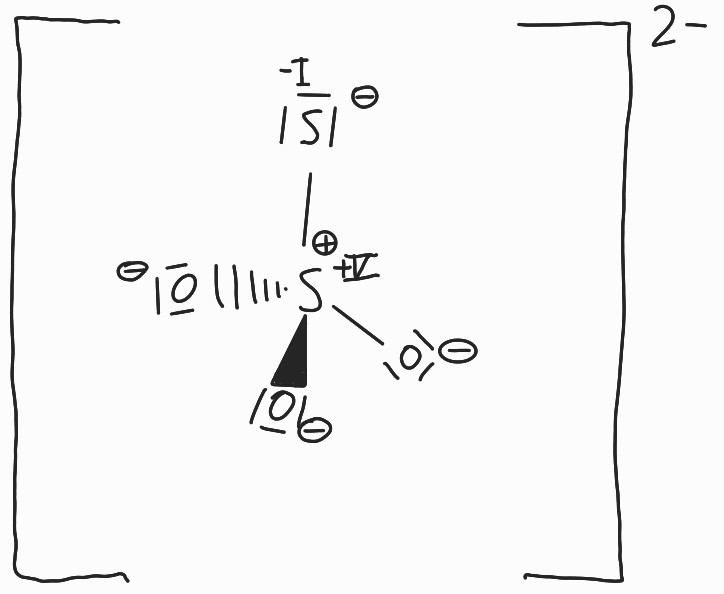
\includegraphics[width=\textwidth]{Bilder/Thiosulfat1.jpg}
        \caption{Strukturformel des Thiosulfat-Ions}
        \label{fig: Thiosulfat}
    \end{minipage}\hfill
    \begin{minipage}{0.48\textwidth}
        \centering
        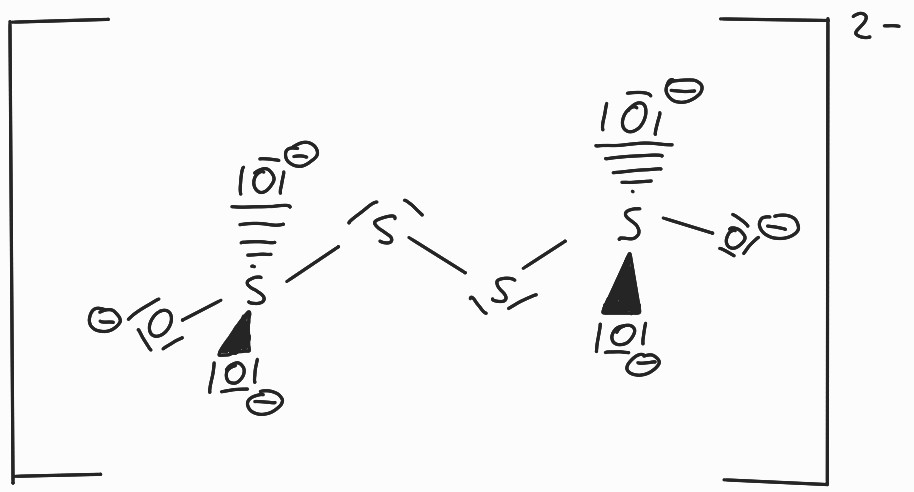
\includegraphics[width=\textwidth]{Bilder/Tetrathionat1.jpg}
        \caption{Strukturformel des Tetrathionat-Ions}
        \label{fig: Tetrathionat}
    \end{minipage}
\end{figure}


\newpage


Am Äquivalenzpunkt ist das Stoffmengenverhältnis von Kupferionen zu den zugegebenen Thiosulfat-Ionen 1 zu 1. Deshalb gilt:
\begin{align*}
    \frac{n(\ce{Cu^{2+}})}{n(\ce{S2O3^{2-}})} &= \frac{2}{2} \Longrightarrow n(\ce{Cu^{2+}}) = n(\ce{S2O3^{2-}})\\[2mm]
    n(\ce{Cu^{2+}}) &= c(\ce{S2O3^{2-}}) \cdot V(\ce{S2O3^{2-}})\\[2mm]
    n(\ce{Cu^{2+}}) &= 0,1\,\frac{{\text{mol}}}{{\text{L}}} \cdot 3,25\,\text{mL}\\[2mm]
    n(\ce{Cu^{2+}}) &= 0,325\,\text{mmol}
\end{align*}

Da nur 25 mL und nicht die ganzen 100 mL der Analyselösung für die Titration verwendet wurden, muss die ausgerechnete Stoffmenge noch mit dem Aliquotenfaktor
\begin{equation}
    F_A = \frac{100\,\text{mL}}{25\,\text{mL}} = 4
\end{equation}

multipliziert werden. Die Stoffmenge der Bromid-Ionen im Analysekolben betrug also:
\begin{equation}
    n_{\text{Probe}} = 4 \cdot 0,325\,\text{mmol} = 1,30\,\text{mmol}
\end{equation}

Das Redoxpaar $\ce{Cu^{2+} + e- <=> Cu^+}$ hat ein Standartelektrodenpotential von 0,16 V \cite{Elektrodenpotentiale} und $\ce{I2 <=> 2I^+ + 2e-}$ von 0,62 V \cite{Elektrodenpotentiale}. Es sollte theoretisch zu keiner Reaktion kommen, da Iod ein höheres Standartelektrodenpotential als die Kupfer-Ionen hat und diese oxidieren sollte. Eine Reaktion findet aber trotzdem statt, da gebildete Kupfer(I)-Ionen mit Iodid als Kupferiodid ausfallen und so dem Gleichgewicht entzogen werden. Das Gleichgewicht reagiert darauf mit Bildung neuer Kupfer(I)-Ionen, die ebenfalls ausfallen.\\


\subsection{Fehlerbetrachtung}
Bei diesem Versuch ist es zu vielen Menschlichen Fehlern gekommen, weswegen die hohe Abweichung des ermittelten Wertes zu dem Literaturwert von 66,27\% zu erklären ist. Der erste Fehler war, dass die Maßlösung nicht exakt auf die Eichmarke aufgefüllt wurde, sondern deutlich mehr demin. Wasser hinzugegeben wurde. Auch bei der Lösung im Erlmeyerkolben wurde teilweise nicht das exakte Mischverhältnis erziehlt, da viele angaben Lauteten "eine Spachtelspitze" oder "einige Tropfen". Zunächst färbte sich die Lösung nach Zugabe der Stärke nicht Blau, sondern hatte eine milchige Farbe, die eigentlich am ende der Titartion hätte auftreten sollen. Auch bei der Titartion kann es zu fehlern gekommen sein, da sich die Lösung zu schnell von dunkelblau zu milchig weiß verfärbt hat und nach ein paar Sekunden wieder blau geworden ist, wodurch es schwierig war, den Äquivalenzpunkt exakt zu bestimmen. Auch das Ablesen nach der Titartion war aufgrund der Beschaffenheit einer Bürette nicht absolut korrekt bestimmbar. Noch dazu wurde aufgrund der fortgeschrittenen Zeit nur ein Titrationsversuch durchgeführt, wodurch die Fehler nicht durch weitere Versuche ausgeglichen werden konnten.\\
Die prozentuale Abweichung der ermittelten Stoffmenge von der Sollstoffmenge von 3,854 mmol beträgt:
\begin{align*}
    \Delta n &= \left(1 - \frac{n_{\ce{Cu^-}}(\text{ist})}{n_{\ce{Cu^-}}(\text{soll})} \right) \cdot 100\\
    \Delta n &= \left( 1 - \frac{1,30\,\text{mmol}}{3,854\,\text{mmol}} \right) \cdot 100\\ 
    \Delta n &= 66,27\% 
\end{align*}
Die prozentuale Abweichung der Stoffmenge beträgt 66,27\%, was auf die vielen Fehlerquellen zurückzuführen ist.


\section{Zusammenfassung}
In Versuch 1 wurden verschiedene Redoxpaare durch Reaktionen mit unterschiedlichenSäuren in die elektrochemische Spannungsreihe eingeordnet.\\

In Versuch 2 wurde die Abhängigkeit des Redoxpotenzial vom pH-Wert anhand der Reaktion von Eisensulfat mit Kaliumnitrat untersucht.\\

In Versuch 3 wurde mithilfe von verschiedenen Versuchen die amphotere Eigenschaft des Wasserstoffperoxids und die Kom- sowie Disproportionierungsreaktion aufgezeigt.\\

In Versuch 4 wurde die Stoffmenge von Kupferionen über eine iodometrische Rücktitration bestimmt. Die Stoffmenge betrug 1,30 mmol, die Abweichung zu der tatsächlichenSollstoffmenge von 3,854 mmol betrug 66,27\%.

\newpage
\renewcommand{\thepage}{\roman{page}}\setcounter{page}{1}
\printbibliography
\end{document}